\documentclass[10pt,landscape]{article}
\usepackage[T1]{fontenc}
\usepackage{lmodern}
\usepackage[margin=0.65in]{geometry}
\usepackage{graphicx,booktabs,longtable,array,microtype,url}
\usepackage[hidelinks]{hyperref}
\emergencystretch=1em
\title{Receiver Adaptation Under Unseen-Receiver Shift\\Supplementary Evidence v0}
\author{OpenEW-SA internal-review draft}\date{}
\begin{document}\maketitle
\section{Scope and Reading Rules}
All rows derive from the frozen six-class WiSig V2 receiver-LOSO protocol. Receivers receive equal weight after averaging five seeds. The evidence CSV retains secondary metrics and other controls. The manuscript distinguishes source-only (R0), unlabeled support (R1), and labeled-support oracle (R2). No packet-level inferential resampling is performed. Later T3A inference is not independent confirmation because prior WiSig findings were known.
\section{Hardware-Family Descriptions}
\setcounter{figure}{6}
\begin{figure}[ht]\centering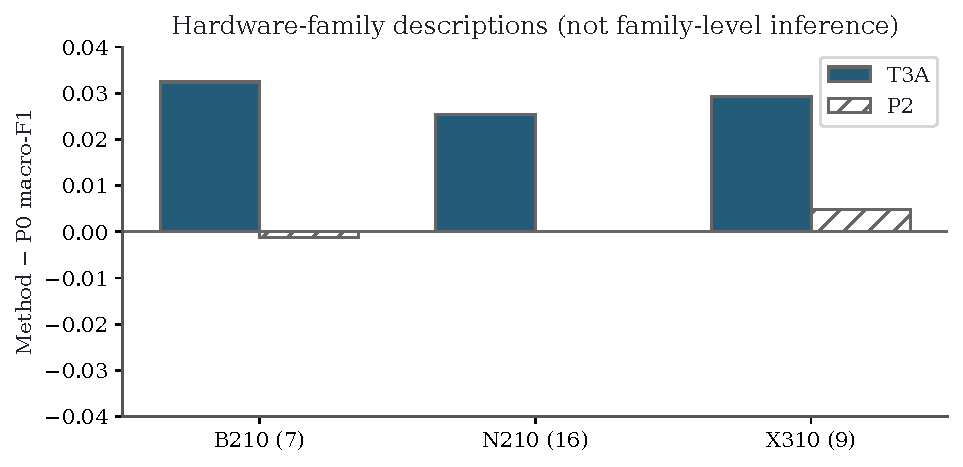
\includegraphics[width=.72\textwidth]{figures/fig07_hardware}\caption{Descriptive hardware-family differences; no family-level inferential claim.}\end{figure}
T3A's mean improvement appears in each observed family; P2 differences are smaller and mixed. Three families cannot establish population-level family generality.
\section{Evidence Progression}
\begin{figure}[ht]\centering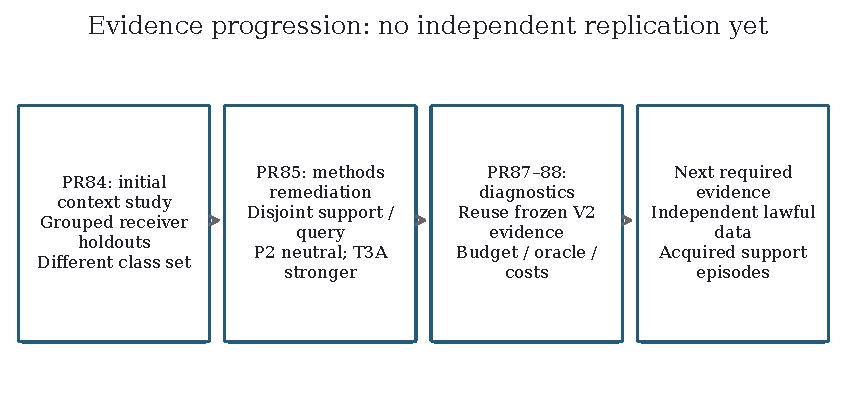
\includegraphics[width=.85\textwidth]{figures/fig08_progression}\caption{Evidence progression, not independent cross-dataset replication.}\end{figure}
These stages are not independent replications. Initial and V2 class sets differ. Query-coupling inference cannot reconstruct every difference between studies.
\section{Post-Hoc Mechanism Findings}
The addendum CSVs retain natural, query-coupled, full-partition context, shuffled-context training, oracle composition, and all support budgets. Same-class-excluded, same-class-only, and transmitter-pure support is label-dependent and non-deployable. The condition NULL remains a string, not a missing value. Equalized matched-ID analysis was ineligible; no performance is manufactured.
\section{Probability and Compute Caveats}
ECE, NLL, and entropy are separate, target-untuned diagnostics. Compute records distinguish source training from reused-checkpoint evaluation; missing isolated components remain missing.
\section{Full Receiver--Seed Lookup}
\small
\begin{longtable}{llrrrrrrrrrr}
\caption{All primary receiver--seed macro-F1 values (six decimals).}\\
Receiver & Seed & P0 & T3A & P2 & P0\_WIDE & P1 & RX\_NORM & DG\_CORAL & DG\_DANN & DG\_GROUPDRO & SUP\_FT\_128\\ \hline \endfirsthead
Receiver & Seed & P0 & T3A & P2 & P0\_WIDE & P1 & RX\_NORM & DG\_CORAL & DG\_DANN & DG\_GROUPDRO & SUP\_FT\_128\\ \hline \endhead
1-1 & 829 & 0.762557 & 0.796521 & 0.816130 & 0.811171 & 0.820377 & 0.731683 & 0.723883 & 0.765954 & 0.672361 & 0.796705\\
1-1 & 1829 & 0.780236 & 0.793835 & 0.841895 & 0.852790 & 0.847741 & 0.778377 & 0.808352 & 0.781049 & 0.738819 & 0.795528\\
1-1 & 2829 & 0.724643 & 0.764187 & 0.840097 & 0.785901 & 0.810470 & 0.725516 & 0.788241 & 0.748486 & 0.800053 & 0.768305\\
1-1 & 3829 & 0.869574 & 0.869418 & 0.822802 & 0.808363 & 0.867455 & 0.837840 & 0.865666 & 0.816339 & 0.771005 & 0.878487\\
1-1 & 4829 & 0.835095 & 0.854666 & 0.813729 & 0.816629 & 0.889589 & 0.857987 & 0.843485 & 0.842374 & 0.815794 & 0.867242\\
1-19 & 829 & 0.651535 & 0.696121 & 0.716672 & 0.688410 & 0.693735 & 0.653114 & 0.651260 & 0.685138 & 0.634783 & 0.692983\\
1-19 & 1829 & 0.759518 & 0.787633 & 0.677157 & 0.633548 & 0.684302 & 0.749123 & 0.752583 & 0.717799 & 0.651088 & 0.774871\\
1-19 & 2829 & 0.679857 & 0.725016 & 0.727288 & 0.748655 & 0.717087 & 0.721395 & 0.687990 & 0.718276 & 0.683804 & 0.708331\\
1-19 & 3829 & 0.708547 & 0.715828 & 0.717579 & 0.704044 & 0.774020 & 0.702019 & 0.725089 & 0.718725 & 0.689780 & 0.731845\\
1-19 & 4829 & 0.740559 & 0.764042 & 0.767678 & 0.791592 & 0.713184 & 0.742981 & 0.732809 & 0.791875 & 0.701710 & 0.773158\\
1-20 & 829 & 0.826851 & 0.847396 & 0.845431 & 0.871346 & 0.869876 & 0.784162 & 0.818376 & 0.849453 & 0.808083 & 0.885683\\
1-20 & 1829 & 0.803390 & 0.861699 & 0.821314 & 0.853110 & 0.887359 & 0.776029 & 0.795136 & 0.824627 & 0.739342 & 0.867261\\
1-20 & 2829 & 0.806609 & 0.851537 & 0.885057 & 0.884453 & 0.875879 & 0.794917 & 0.796487 & 0.776394 & 0.753288 & 0.857819\\
1-20 & 3829 & 0.742166 & 0.766201 & 0.882056 & 0.715025 & 0.838184 & 0.676769 & 0.753969 & 0.788885 & 0.661323 & 0.802975\\
1-20 & 4829 & 0.837229 & 0.873641 & 0.850209 & 0.845167 & 0.859643 & 0.860391 & 0.863850 & 0.849508 & 0.744699 & 0.887199\\
13-14 & 829 & 0.744347 & 0.808511 & 0.731523 & 0.764823 & 0.786259 & 0.665911 & 0.763925 & 0.734980 & 0.684805 & 0.809917\\
13-14 & 1829 & 0.716908 & 0.771564 & 0.725656 & 0.607496 & 0.765723 & 0.630861 & 0.682513 & 0.712711 & 0.607831 & 0.780750\\
13-14 & 2829 & 0.821165 & 0.897804 & 0.799494 & 0.709008 & 0.780895 & 0.801589 & 0.845021 & 0.823416 & 0.665906 & 0.871870\\
13-14 & 3829 & 0.611546 & 0.663427 & 0.656755 & 0.603355 & 0.628412 & 0.586723 & 0.605937 & 0.572728 & 0.564055 & 0.635204\\
13-14 & 4829 & 0.710391 & 0.768553 & 0.692360 & 0.691772 & 0.730489 & 0.626209 & 0.667709 & 0.749630 & 0.635571 & 0.811673\\
13-7 & 829 & 0.832344 & 0.829815 & 0.824295 & 0.798201 & 0.826434 & 0.822214 & 0.819162 & 0.801065 & 0.805855 & 0.844212\\
13-7 & 1829 & 0.848900 & 0.825768 & 0.812873 & 0.839261 & 0.788505 & 0.819581 & 0.842240 & 0.814632 & 0.811001 & 0.855988\\
13-7 & 2829 & 0.810596 & 0.816867 & 0.818871 & 0.834245 & 0.800162 & 0.820708 & 0.837304 & 0.799480 & 0.811824 & 0.823353\\
13-7 & 3829 & 0.788397 & 0.790026 & 0.818534 & 0.792262 & 0.752609 & 0.757695 & 0.800678 & 0.758643 & 0.792625 & 0.806078\\
13-7 & 4829 & 0.844311 & 0.821462 & 0.783236 & 0.849478 & 0.827991 & 0.844484 & 0.839425 & 0.836108 & 0.766677 & 0.852867\\
14-7 & 829 & 0.864940 & 0.932698 & 0.881742 & 0.885475 & 0.863674 & 0.934775 & 0.876381 & 0.862904 & 0.847059 & 0.923209\\
14-7 & 1829 & 0.864394 & 0.900957 & 0.788252 & 0.836539 & 0.818822 & 0.856781 & 0.874378 & 0.807130 & 0.835491 & 0.893307\\
14-7 & 2829 & 0.876880 & 0.916952 & 0.861088 & 0.888976 & 0.843211 & 0.924947 & 0.892995 & 0.897403 & 0.763214 & 0.924511\\
14-7 & 3829 & 0.843113 & 0.892149 & 0.834337 & 0.806144 & 0.850437 & 0.854617 & 0.817273 & 0.846609 & 0.844778 & 0.886440\\
14-7 & 4829 & 0.914606 & 0.947781 & 0.906455 & 0.906947 & 0.878796 & 0.879672 & 0.922833 & 0.895456 & 0.823703 & 0.946507\\
18-19 & 829 & 0.804243 & 0.835252 & 0.813705 & 0.813301 & 0.819219 & 0.792828 & 0.815660 & 0.780318 & 0.774161 & 0.826445\\
18-19 & 1829 & 0.826814 & 0.842525 & 0.827084 & 0.817944 & 0.844977 & 0.831001 & 0.807751 & 0.822248 & 0.828492 & 0.833242\\
18-19 & 2829 & 0.834359 & 0.851111 & 0.831691 & 0.845324 & 0.816695 & 0.839760 & 0.842188 & 0.849890 & 0.834519 & 0.838141\\
18-19 & 3829 & 0.809083 & 0.822855 & 0.843617 & 0.774737 & 0.822494 & 0.798705 & 0.807537 & 0.795535 & 0.740715 & 0.812024\\
18-19 & 4829 & 0.783426 & 0.802897 & 0.800542 & 0.816382 & 0.784534 & 0.818312 & 0.813402 & 0.799459 & 0.794818 & 0.794971\\
18-2 & 829 & 0.745066 & 0.756714 & 0.778264 & 0.765435 & 0.788067 & 0.751887 & 0.768743 & 0.776589 & 0.692934 & 0.797476\\
18-2 & 1829 & 0.797835 & 0.792423 & 0.820797 & 0.819734 & 0.770351 & 0.811182 & 0.808986 & 0.782553 & 0.741514 & 0.846300\\
18-2 & 2829 & 0.767784 & 0.799950 & 0.793808 & 0.761845 & 0.788324 & 0.769410 & 0.768405 & 0.737525 & 0.691755 & 0.809178\\
18-2 & 3829 & 0.750066 & 0.805171 & 0.815649 & 0.826007 & 0.774541 & 0.757608 & 0.791337 & 0.794803 & 0.722909 & 0.771633\\
18-2 & 4829 & 0.743846 & 0.790388 & 0.801752 & 0.765883 & 0.777895 & 0.726916 & 0.729001 & 0.707913 & 0.691961 & 0.798227\\
19-1 & 829 & 0.783869 & 0.814720 & 0.780557 & 0.785509 & 0.781291 & 0.735409 & 0.733805 & 0.775134 & 0.714710 & 0.798543\\
19-1 & 1829 & 0.769662 & 0.808177 & 0.667332 & 0.761146 & 0.748279 & 0.802094 & 0.778332 & 0.779827 & 0.690429 & 0.798284\\
19-1 & 2829 & 0.745915 & 0.803538 & 0.795150 & 0.732152 & 0.794223 & 0.748402 & 0.746582 & 0.747937 & 0.666539 & 0.752471\\
19-1 & 3829 & 0.752564 & 0.774395 & 0.772431 & 0.803091 & 0.742738 & 0.724524 & 0.729183 & 0.761184 & 0.678694 & 0.781892\\
19-1 & 4829 & 0.784432 & 0.803446 & 0.778109 & 0.780224 & 0.739781 & 0.802122 & 0.811128 & 0.800713 & 0.725523 & 0.809960\\
19-19 & 829 & 0.865722 & 0.915086 & 0.827504 & 0.892998 & 0.912459 & 0.845009 & 0.867694 & 0.871270 & 0.813619 & 0.897682\\
19-19 & 1829 & 0.864183 & 0.926533 & 0.811536 & 0.810275 & 0.811031 & 0.875056 & 0.818697 & 0.854496 & 0.808529 & 0.918708\\
19-19 & 2829 & 0.868426 & 0.923727 & 0.835156 & 0.920996 & 0.868156 & 0.921185 & 0.864124 & 0.879525 & 0.817692 & 0.918567\\
19-19 & 3829 & 0.791444 & 0.849495 & 0.829281 & 0.757791 & 0.748215 & 0.759941 & 0.757134 & 0.716895 & 0.728539 & 0.839205\\
19-19 & 4829 & 0.904781 & 0.937552 & 0.798883 & 0.870090 & 0.811622 & 0.893983 & 0.871860 & 0.884298 & 0.864895 & 0.936393\\
19-2 & 829 & 0.773136 & 0.784322 & 0.693007 & 0.893838 & 0.855750 & 0.757040 & 0.788770 & 0.739706 & 0.682507 & 0.792490\\
19-2 & 1829 & 0.819992 & 0.845619 & 0.836055 & 0.827619 & 0.791773 & 0.812872 & 0.825462 & 0.809240 & 0.705337 & 0.835731\\
19-2 & 2829 & 0.812693 & 0.834217 & 0.759583 & 0.834580 & 0.763352 & 0.799967 & 0.816001 & 0.852331 & 0.754270 & 0.836812\\
19-2 & 3829 & 0.801746 & 0.825870 & 0.852835 & 0.864980 & 0.860755 & 0.816287 & 0.802236 & 0.809976 & 0.767777 & 0.837473\\
19-2 & 4829 & 0.869519 & 0.920660 & 0.864280 & 0.836293 & 0.867463 & 0.903148 & 0.895325 & 0.881912 & 0.849377 & 0.909068\\
19-20 & 829 & 0.815949 & 0.792164 & 0.778830 & 0.794322 & 0.778467 & 0.857003 & 0.821376 & 0.851151 & 0.771307 & 0.857203\\
19-20 & 1829 & 0.825958 & 0.838749 & 0.793357 & 0.765694 & 0.756925 & 0.828220 & 0.827503 & 0.817360 & 0.770954 & 0.858499\\
19-20 & 2829 & 0.847020 & 0.855951 & 0.773796 & 0.729421 & 0.729707 & 0.811414 & 0.773278 & 0.820450 & 0.780755 & 0.858700\\
19-20 & 3829 & 0.728678 & 0.734746 & 0.799727 & 0.712079 & 0.749568 & 0.718309 & 0.737321 & 0.751411 & 0.717417 & 0.759061\\
19-20 & 4829 & 0.726779 & 0.743491 & 0.745954 & 0.693517 & 0.747191 & 0.711018 & 0.717224 & 0.718228 & 0.699305 & 0.744506\\
2-1 & 829 & 0.796905 & 0.770560 & 0.800329 & 0.800156 & 0.793774 & 0.809093 & 0.808401 & 0.803585 & 0.715148 & 0.845650\\
2-1 & 1829 & 0.768650 & 0.809463 & 0.798981 & 0.877294 & 0.776490 & 0.823701 & 0.809121 & 0.846904 & 0.771964 & 0.799036\\
2-1 & 2829 & 0.714120 & 0.772439 & 0.781113 & 0.811439 & 0.850736 & 0.768567 & 0.722392 & 0.794578 & 0.758356 & 0.770819\\
2-1 & 3829 & 0.808415 & 0.814006 & 0.823862 & 0.758186 & 0.818388 & 0.827886 & 0.795301 & 0.765892 & 0.763858 & 0.821742\\
2-1 & 4829 & 0.819628 & 0.821854 & 0.763172 & 0.811373 & 0.786602 & 0.821615 & 0.805793 & 0.805541 & 0.759938 & 0.848830\\
2-19 & 829 & 0.809458 & 0.848791 & 0.846191 & 0.873556 & 0.919059 & 0.790859 & 0.786895 & 0.835163 & 0.733466 & 0.866527\\
2-19 & 1829 & 0.923883 & 0.936290 & 0.822530 & 0.831108 & 0.895378 & 0.911149 & 0.903635 & 0.875119 & 0.870682 & 0.935151\\
2-19 & 2829 & 0.852022 & 0.860694 & 0.883098 & 0.862718 & 0.810207 & 0.779282 & 0.832408 & 0.863321 & 0.832133 & 0.873448\\
2-19 & 3829 & 0.840100 & 0.871437 & 0.835390 & 0.825191 & 0.879882 & 0.891122 & 0.848733 & 0.879630 & 0.809802 & 0.895083\\
2-19 & 4829 & 0.854468 & 0.878507 & 0.897767 & 0.850346 & 0.895172 & 0.834682 & 0.880186 & 0.843491 & 0.761453 & 0.922139\\
20-1 & 829 & 0.940723 & 0.948180 & 0.947252 & 0.933655 & 0.941161 & 0.947203 & 0.938316 & 0.934413 & 0.896955 & 0.950857\\
20-1 & 1829 & 0.927371 & 0.934958 & 0.899259 & 0.908296 & 0.955359 & 0.933333 & 0.924674 & 0.938581 & 0.881197 & 0.942973\\
20-1 & 2829 & 0.914419 & 0.913371 & 0.952753 & 0.916285 & 0.917257 & 0.908111 & 0.895294 & 0.893164 & 0.812355 & 0.926030\\
20-1 & 3829 & 0.881511 & 0.906053 & 0.952151 & 0.907721 & 0.913488 & 0.896003 & 0.905702 & 0.893559 & 0.856561 & 0.900552\\
20-1 & 4829 & 0.911074 & 0.929046 & 0.888126 & 0.910812 & 0.882786 & 0.943079 & 0.905506 & 0.890112 & 0.880540 & 0.930214\\
20-19 & 829 & 0.861621 & 0.896296 & 0.879039 & 0.878362 & 0.921234 & 0.881776 & 0.848493 & 0.880075 & 0.776696 & 0.916554\\
20-19 & 1829 & 0.926169 & 0.934636 & 0.811544 & 0.904114 & 0.889506 & 0.921806 & 0.951346 & 0.915351 & 0.815574 & 0.957965\\
20-19 & 2829 & 0.863648 & 0.897124 & 0.829203 & 0.912142 & 0.769683 & 0.861610 & 0.876275 & 0.863041 & 0.798084 & 0.921930\\
20-19 & 3829 & 0.841492 & 0.873088 & 0.861600 & 0.848766 & 0.875137 & 0.848955 & 0.857128 & 0.869854 & 0.779574 & 0.841533\\
20-19 & 4829 & 0.927237 & 0.931466 & 0.848672 & 0.916485 & 0.830456 & 0.936565 & 0.891068 & 0.961630 & 0.856884 & 0.940365\\
20-20 & 829 & 0.847880 & 0.875811 & 0.813231 & 0.802523 & 0.796242 & 0.811860 & 0.821630 & 0.806974 & 0.791490 & 0.883326\\
20-20 & 1829 & 0.704573 & 0.778253 & 0.748911 & 0.699571 & 0.730173 & 0.751393 & 0.785666 & 0.679208 & 0.692434 & 0.758623\\
20-20 & 2829 & 0.761770 & 0.801209 & 0.797279 & 0.713011 & 0.725482 & 0.797732 & 0.795402 & 0.779018 & 0.719301 & 0.804473\\
20-20 & 3829 & 0.730581 & 0.745813 & 0.800690 & 0.746773 & 0.774403 & 0.735922 & 0.730007 & 0.734417 & 0.675505 & 0.766896\\
20-20 & 4829 & 0.776082 & 0.799145 & 0.750381 & 0.749952 & 0.745475 & 0.749186 & 0.793070 & 0.739020 & 0.767942 & 0.817452\\
23-1 & 829 & 0.917912 & 0.935668 & 0.907680 & 0.883261 & 0.908980 & 0.915585 & 0.905201 & 0.926645 & 0.903689 & 0.932656\\
23-1 & 1829 & 0.938284 & 0.941454 & 0.907601 & 0.935898 & 0.903510 & 0.901316 & 0.950560 & 0.919879 & 0.890832 & 0.946105\\
23-1 & 2829 & 0.908765 & 0.917035 & 0.895416 & 0.903525 & 0.886513 & 0.896085 & 0.916592 & 0.894863 & 0.883017 & 0.933770\\
23-1 & 3829 & 0.893326 & 0.906681 & 0.926626 & 0.905910 & 0.921862 & 0.876244 & 0.904834 & 0.877396 & 0.867474 & 0.910666\\
23-1 & 4829 & 0.917152 & 0.942282 & 0.933020 & 0.904404 & 0.921469 & 0.901971 & 0.903236 & 0.906303 & 0.870199 & 0.939356\\
23-3 & 829 & 0.888059 & 0.904480 & 0.811478 & 0.834718 & 0.870785 & 0.871879 & 0.820635 & 0.832183 & 0.868436 & 0.926003\\
23-3 & 1829 & 0.856228 & 0.902783 & 0.876034 & 0.795228 & 0.876846 & 0.844211 & 0.848156 & 0.806448 & 0.823978 & 0.914888\\
23-3 & 2829 & 0.900558 & 0.912660 & 0.872689 & 0.805094 & 0.881926 & 0.860608 & 0.865631 & 0.877431 & 0.865910 & 0.941422\\
23-3 & 3829 & 0.778176 & 0.808454 & 0.839098 & 0.794310 & 0.822017 & 0.765488 & 0.744648 & 0.757924 & 0.787725 & 0.856594\\
23-3 & 4829 & 0.856967 & 0.884135 & 0.832193 & 0.799446 & 0.878535 & 0.785342 & 0.799252 & 0.822536 & 0.812875 & 0.901688\\
23-5 & 829 & 0.870369 & 0.878097 & 0.851257 & 0.864320 & 0.825313 & 0.837950 & 0.865180 & 0.853459 & 0.765638 & 0.893464\\
23-5 & 1829 & 0.814424 & 0.838705 & 0.765332 & 0.832439 & 0.850020 & 0.802779 & 0.815081 & 0.818691 & 0.740077 & 0.851732\\
23-5 & 2829 & 0.841528 & 0.863006 & 0.785657 & 0.856033 & 0.813698 & 0.831207 & 0.840698 & 0.838716 & 0.782980 & 0.864429\\
23-5 & 3829 & 0.766735 & 0.792269 & 0.789386 & 0.759972 & 0.785840 & 0.761332 & 0.768387 & 0.753050 & 0.741062 & 0.802045\\
23-5 & 4829 & 0.827636 & 0.838574 & 0.838172 & 0.838083 & 0.827429 & 0.823445 & 0.844985 & 0.836448 & 0.792614 & 0.854437\\
23-6 & 829 & 0.880755 & 0.918592 & 0.898453 & 0.881827 & 0.893791 & 0.875155 & 0.896206 & 0.872912 & 0.865616 & 0.922227\\
23-6 & 1829 & 0.921344 & 0.962863 & 0.917052 & 0.884070 & 0.902515 & 0.917313 & 0.918825 & 0.888911 & 0.896656 & 0.954561\\
23-6 & 2829 & 0.924948 & 0.948478 & 0.895428 & 0.873269 & 0.900421 & 0.913214 & 0.919570 & 0.902616 & 0.939621 & 0.956062\\
23-6 & 3829 & 0.872496 & 0.887310 & 0.936345 & 0.903493 & 0.915037 & 0.823581 & 0.832423 & 0.858117 & 0.828389 & 0.901159\\
23-6 & 4829 & 0.906527 & 0.942971 & 0.932748 & 0.891397 & 0.927948 & 0.930986 & 0.900514 & 0.922754 & 0.927358 & 0.946418\\
23-7 & 829 & 0.725702 & 0.739526 & 0.715259 & 0.738510 & 0.775487 & 0.748582 & 0.743422 & 0.723620 & 0.695420 & 0.765616\\
23-7 & 1829 & 0.732291 & 0.786975 & 0.757994 & 0.726161 & 0.741801 & 0.731047 & 0.732804 & 0.753985 & 0.688267 & 0.770748\\
23-7 & 2829 & 0.700684 & 0.719704 & 0.762861 & 0.675818 & 0.703446 & 0.745584 & 0.705962 & 0.739641 & 0.707201 & 0.752112\\
23-7 & 3829 & 0.686098 & 0.735105 & 0.726793 & 0.735377 & 0.756455 & 0.699703 & 0.695902 & 0.695949 & 0.651160 & 0.745749\\
23-7 & 4829 & 0.702046 & 0.653853 & 0.775268 & 0.743954 & 0.748293 & 0.698675 & 0.702633 & 0.718087 & 0.647903 & 0.749545\\
24-13 & 829 & 0.856099 & 0.902943 & 0.885443 & 0.869933 & 0.859742 & 0.832610 & 0.848324 & 0.815180 & 0.798137 & 0.897018\\
24-13 & 1829 & 0.833905 & 0.876711 & 0.846648 & 0.818257 & 0.865779 & 0.843192 & 0.842744 & 0.830280 & 0.839674 & 0.885621\\
24-13 & 2829 & 0.791007 & 0.823565 & 0.851182 & 0.834623 & 0.849801 & 0.854520 & 0.821948 & 0.849048 & 0.756216 & 0.860129\\
24-13 & 3829 & 0.841597 & 0.871221 & 0.864166 & 0.816320 & 0.814418 & 0.837021 & 0.842919 & 0.835939 & 0.782518 & 0.876339\\
24-13 & 4829 & 0.803580 & 0.861942 & 0.828940 & 0.800559 & 0.829197 & 0.815283 & 0.800091 & 0.813328 & 0.767718 & 0.886730\\
24-16 & 829 & 0.919194 & 0.950406 & 0.930614 & 0.931778 & 0.906150 & 0.855004 & 0.947847 & 0.894043 & 0.845468 & 0.942557\\
24-16 & 1829 & 0.863668 & 0.947470 & 0.820333 & 0.783103 & 0.841984 & 0.825403 & 0.886175 & 0.834455 & 0.863171 & 0.922328\\
24-16 & 2829 & 0.936211 & 0.971788 & 0.823004 & 0.874677 & 0.812879 & 0.868227 & 0.893335 & 0.902316 & 0.885153 & 0.965513\\
24-16 & 3829 & 0.798166 & 0.895455 & 0.862339 & 0.783482 & 0.770641 & 0.774258 & 0.741531 & 0.769419 & 0.723881 & 0.825759\\
24-16 & 4829 & 0.904489 & 0.964125 & 0.825720 & 0.846634 & 0.815555 & 0.904140 & 0.836180 & 0.921600 & 0.790372 & 0.944997\\
24-5 & 829 & 0.550331 & 0.611814 & 0.565240 & 0.582729 & 0.593430 & 0.536841 & 0.547317 & 0.537699 & 0.542340 & 0.564688\\
24-5 & 1829 & 0.554286 & 0.589535 & 0.587519 & 0.564784 & 0.562323 & 0.526355 & 0.558989 & 0.523040 & 0.520210 & 0.564296\\
24-5 & 2829 & 0.558587 & 0.617435 & 0.568227 & 0.486658 & 0.517979 & 0.560634 & 0.538109 & 0.534495 & 0.553852 & 0.584404\\
24-5 & 3829 & 0.560056 & 0.587876 & 0.559820 & 0.561446 & 0.589272 & 0.582376 & 0.563509 & 0.554265 & 0.552117 & 0.591650\\
24-5 & 4829 & 0.575772 & 0.606400 & 0.601755 & 0.581444 & 0.550732 & 0.569866 & 0.568371 & 0.558478 & 0.572617 & 0.612285\\
24-6 & 829 & 0.862978 & 0.876669 & 0.884990 & 0.894263 & 0.906896 & 0.884111 & 0.874241 & 0.837362 & 0.805728 & 0.885724\\
24-6 & 1829 & 0.871695 & 0.891957 & 0.886829 & 0.889808 & 0.856183 & 0.893271 & 0.872567 & 0.828074 & 0.857896 & 0.889917\\
24-6 & 2829 & 0.881151 & 0.883982 & 0.908949 & 0.882649 & 0.880427 & 0.876358 & 0.877291 & 0.877367 & 0.855880 & 0.910068\\
24-6 & 3829 & 0.895274 & 0.910545 & 0.862020 & 0.879945 & 0.919287 & 0.899961 & 0.886137 & 0.845671 & 0.885728 & 0.927310\\
24-6 & 4829 & 0.910904 & 0.914100 & 0.899574 & 0.919445 & 0.877252 & 0.922561 & 0.910067 & 0.902900 & 0.858164 & 0.918351\\
3-19 & 829 & 0.660370 & 0.720588 & 0.692073 & 0.691273 & 0.674644 & 0.661473 & 0.648550 & 0.610754 & 0.671824 & 0.729888\\
3-19 & 1829 & 0.547418 & 0.687580 & 0.587676 & 0.483386 & 0.596169 & 0.510077 & 0.537046 & 0.488922 & 0.672879 & 0.623781\\
3-19 & 2829 & 0.675025 & 0.711563 & 0.614455 & 0.580864 & 0.523123 & 0.653666 & 0.667348 & 0.657539 & 0.695066 & 0.713339\\
3-19 & 3829 & 0.614688 & 0.693595 & 0.602054 & 0.535988 & 0.595649 & 0.599971 & 0.608401 & 0.609261 & 0.602067 & 0.663479\\
3-19 & 4829 & 0.589750 & 0.699087 & 0.530509 & 0.582614 & 0.594502 & 0.629318 & 0.620091 & 0.587943 & 0.740415 & 0.667713\\
7-14 & 829 & 0.729809 & 0.720528 & 0.718702 & 0.702202 & 0.747738 & 0.704141 & 0.718689 & 0.715490 & 0.663734 & 0.746283\\
7-14 & 1829 & 0.778053 & 0.790606 & 0.741244 & 0.774599 & 0.778020 & 0.761900 & 0.754752 & 0.764442 & 0.666044 & 0.787731\\
7-14 & 2829 & 0.720050 & 0.739194 & 0.744130 & 0.758630 & 0.791328 & 0.740017 & 0.742055 & 0.726312 & 0.675430 & 0.742886\\
7-14 & 3829 & 0.718177 & 0.744329 & 0.773009 & 0.756888 & 0.809522 & 0.737279 & 0.707080 & 0.720029 & 0.657969 & 0.735351\\
7-14 & 4829 & 0.865528 & 0.901395 & 0.796592 & 0.823147 & 0.773207 & 0.830408 & 0.836506 & 0.808433 & 0.727925 & 0.887352\\
7-7 & 829 & 0.905247 & 0.908621 & 0.889882 & 0.952288 & 0.918843 & 0.894941 & 0.893452 & 0.876443 & 0.822625 & 0.912349\\
7-7 & 1829 & 0.882548 & 0.903127 & 0.906254 & 0.922923 & 0.909232 & 0.892083 & 0.896729 & 0.895252 & 0.831138 & 0.912089\\
7-7 & 2829 & 0.917111 & 0.935671 & 0.894501 & 0.922890 & 0.919004 & 0.922838 & 0.896704 & 0.927757 & 0.828725 & 0.938863\\
7-7 & 3829 & 0.858316 & 0.866437 & 0.918024 & 0.866230 & 0.848756 & 0.856938 & 0.850363 & 0.846786 & 0.836312 & 0.866312\\
7-7 & 4829 & 0.891185 & 0.901482 & 0.845508 & 0.882297 & 0.906795 & 0.929575 & 0.908084 & 0.918060 & 0.859652 & 0.923625\\
8-14 & 829 & 0.679517 & 0.722304 & 0.676504 & 0.721441 & 0.737461 & 0.690490 & 0.703107 & 0.707321 & 0.619547 & 0.724223\\
8-14 & 1829 & 0.726077 & 0.746949 & 0.681396 & 0.670132 & 0.679508 & 0.670171 & 0.709690 & 0.701823 & 0.650348 & 0.755527\\
8-14 & 2829 & 0.747488 & 0.751132 & 0.677005 & 0.692375 & 0.719052 & 0.722186 & 0.755263 & 0.729234 & 0.666463 & 0.764072\\
8-14 & 3829 & 0.682107 & 0.720420 & 0.673837 & 0.571958 & 0.643995 & 0.654219 & 0.724590 & 0.621818 & 0.634861 & 0.711166\\
8-14 & 4829 & 0.694773 & 0.729197 & 0.684105 & 0.702592 & 0.656423 & 0.688243 & 0.767523 & 0.739655 & 0.699933 & 0.734809\\
8-7 & 829 & 0.844368 & 0.858389 & 0.826263 & 0.838222 & 0.846793 & 0.842907 & 0.856274 & 0.849063 & 0.761640 & 0.841284\\
8-7 & 1829 & 0.831854 & 0.843033 & 0.814726 & 0.807790 & 0.839626 & 0.829806 & 0.804716 & 0.816220 & 0.739220 & 0.841104\\
8-7 & 2829 & 0.839105 & 0.852958 & 0.841500 & 0.817055 & 0.823358 & 0.826123 & 0.832154 & 0.843108 & 0.795393 & 0.839972\\
8-7 & 3829 & 0.769779 & 0.787199 & 0.805742 & 0.828228 & 0.811367 & 0.786304 & 0.763162 & 0.798920 & 0.722087 & 0.789200\\
8-7 & 4829 & 0.838952 & 0.850271 & 0.787537 & 0.840239 & 0.846088 & 0.826809 & 0.842717 & 0.831719 & 0.803493 & 0.846699\\
8-8 & 829 & 0.918554 & 0.940903 & 0.883358 & 0.868935 & 0.925075 & 0.914284 & 0.927442 & 0.881382 & 0.784814 & 0.938851\\
8-8 & 1829 & 0.885206 & 0.900421 & 0.860785 & 0.871341 & 0.932189 & 0.881942 & 0.921409 & 0.899251 & 0.846658 & 0.903079\\
8-8 & 2829 & 0.915039 & 0.932162 & 0.888108 & 0.903250 & 0.935521 & 0.872630 & 0.905448 & 0.890065 & 0.819742 & 0.938441\\
8-8 & 3829 & 0.832639 & 0.860888 & 0.871809 & 0.857544 & 0.905713 & 0.836119 & 0.838684 & 0.846400 & 0.776500 & 0.855488\\
8-8 & 4829 & 0.911876 & 0.920819 & 0.922330 & 0.901964 & 0.922225 & 0.912708 & 0.930802 & 0.926004 & 0.881057 & 0.907477\\
\end{longtable}

\end{document}
